\documentclass[border=1mm]{standalone}
\usepackage{tikz}
\begin{document}
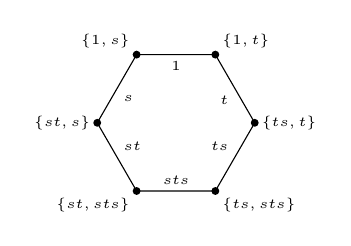
\begin{tikzpicture}
	\tiny
	\coordinate (a) at (120:1);
	\coordinate (b) at (180:1);
	\coordinate (c) at (240:1);
	\coordinate (d) at (300:1);
	\coordinate (e) at (360:1);
	\coordinate (f) at (60:1);

\fill (a) circle (0.05);
\fill (b) circle (0.05);
\fill (c) circle (0.05);
\fill (d) circle (0.05);
\fill (e) circle (0.05);
\fill (f) circle (0.05);

	\draw (a) -- (b) node[pos=0,above left]{$\{1,s\}$} node[pos=0.5,below right]{$s$} -- (c) node[pos=0,left]{$\{st,s\}$} node[pos=0.5,above right]{$st$} -- (d)node[pos=0,below left]{$\{st,sts\}$} node[pos=0.5,above]{$sts$} -- (e)node[pos=0,below right]{$\{ts,sts\}$} node[pos=0.5,above left]{$ts$} -- (f)node[pos=0,right]{$\{ts,t\}$} node[pos=0.5,below left]{$t$} -- (a)node[pos=0,above right]{$\{1,t\}$} node[pos=0.5,below]{$1$};
\end{tikzpicture}
\end{document}
